\section{Background: What is Serialism?}

In general, serialism is a musical composition technique where a set of values, chosen through some methodical process, 
generates a sequence of musical elements. Its origins are often attributed to Arnold Schoenberg's twelve-tone technique, which
he began to use in the 1920s. In this system, each note in the chromatic scale is assigned an integer value, giving us a set of twelve
``pitch classes'' (Figure~\ref{fig:pc}).
A composer utilizing this method then takes each of these integers, and orders them into a $twelve$ $tone$ $row$, where 
each number appears exactly once. We refer to this row as the $prime form$ of a piece, and conventionally refer 
to it as $P_0$. 

\begin{figure}
\begin{minipage}{0.6\textwidth}
	\centering
	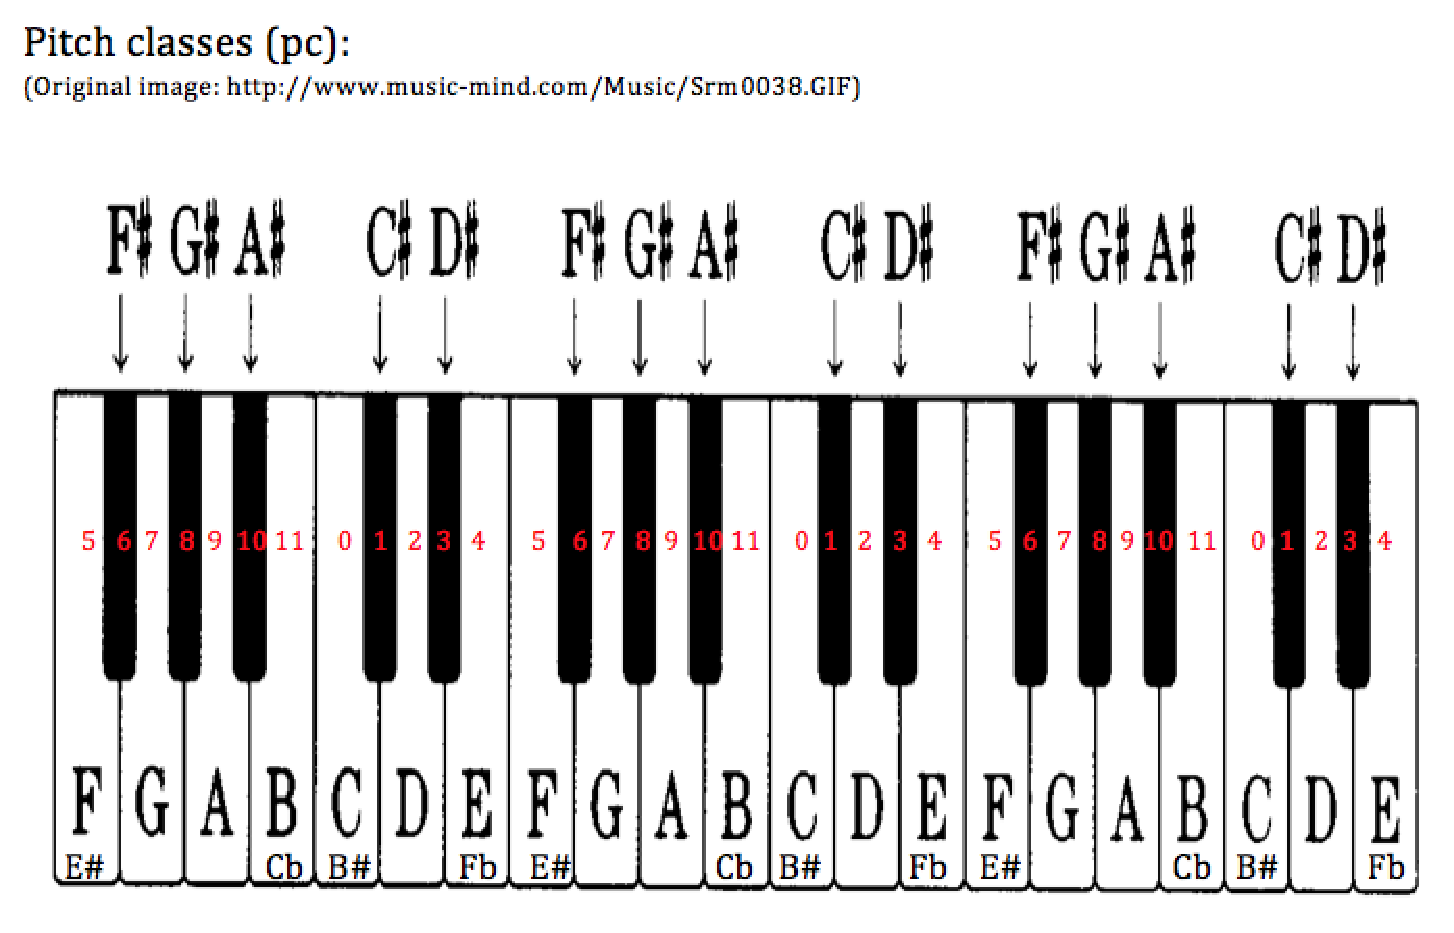
\includegraphics[width=\textwidth]{figures/serialismPianoImage}
	\caption{pitch classes}
	\label{fig:pc}
\end{minipage}\hfill
\begin{minipage}{0.4\textwidth}
	\centering
		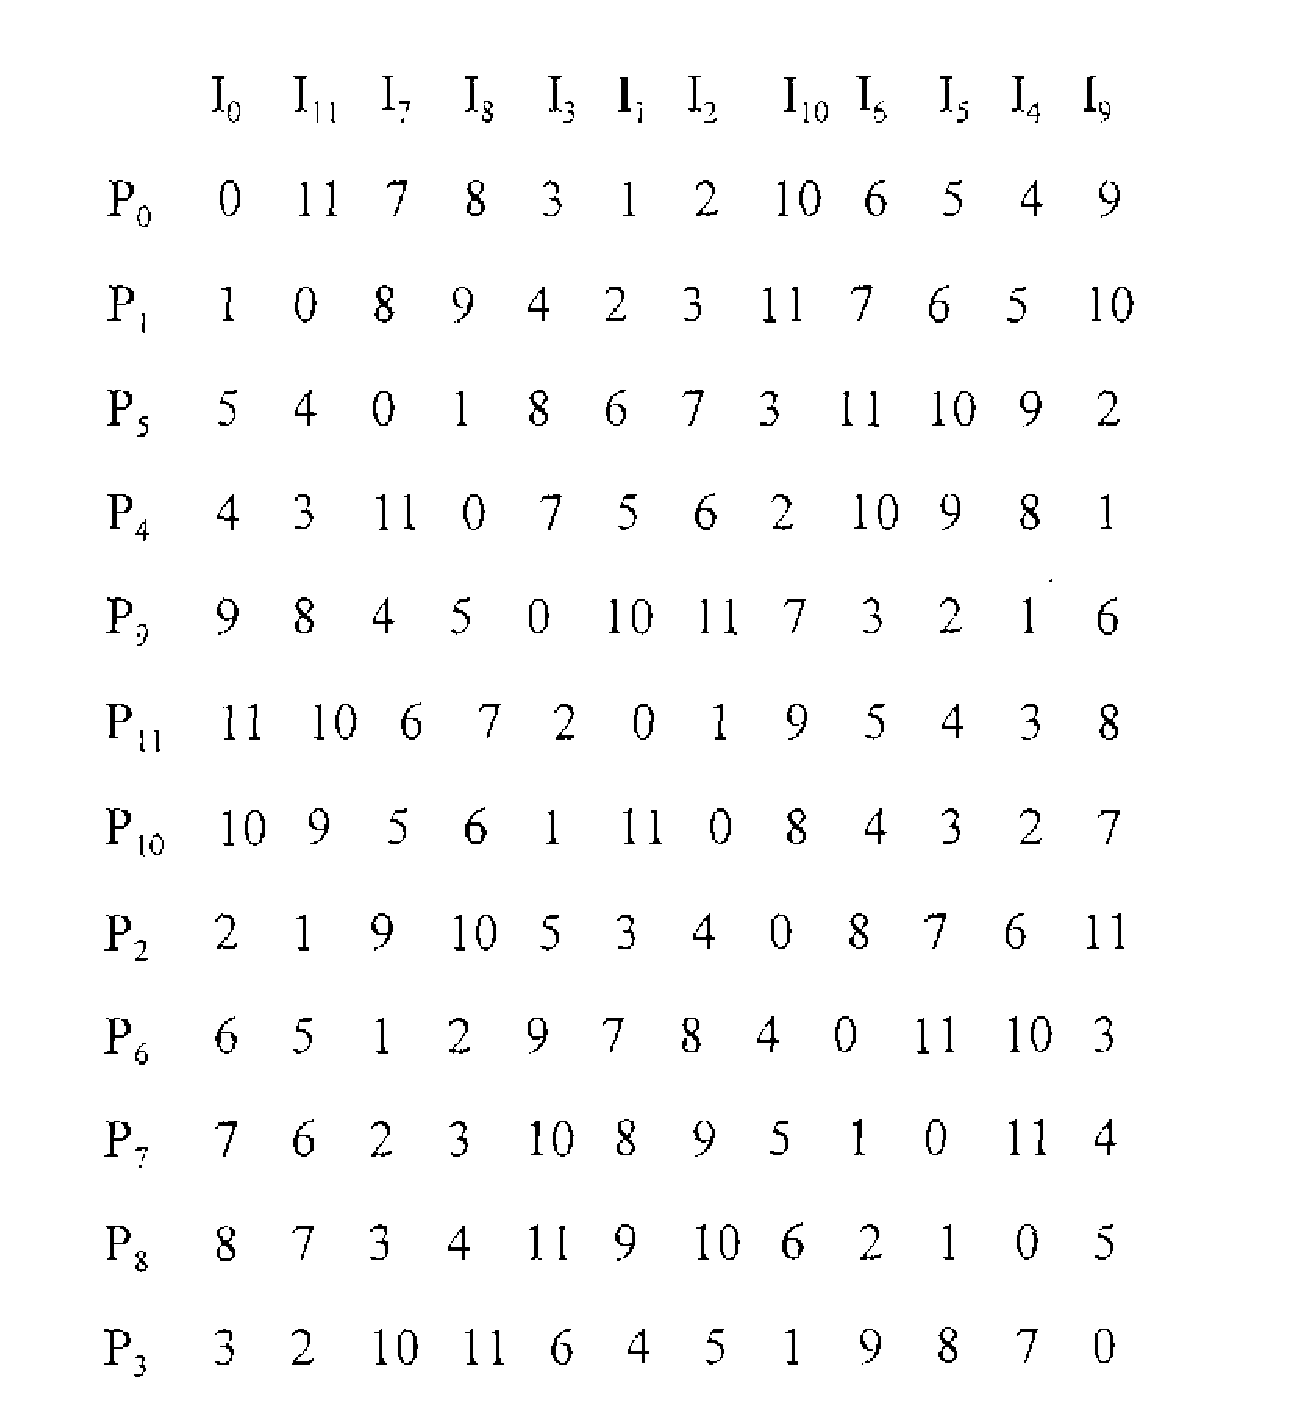
\includegraphics[width=\textwidth]{figures/12_tone}
	\caption{twelve tone matrix}
	\label{fig:12tone}
\end{minipage}
\end{figure}


The composer can then generate other rows that are derived from $P_0$ through three types of transformations:
transposition, inversion, and retrograde. In each of these transformations, we always use mod 12 arithmetic to preserve the 
numbering system of our pitch classes. Transposing a row consists of taking each pitch class in the row and adding the same number 
to each. If we transpose $P_0$ by four semitones, we add four mod twelve to each pitch class in $P_0$ and end up with a new row 
called $P_4$. In general, $P_x$ is a transposition of $P_0$ by $x$ semitones. To invert a row, we "flip" each interval between two 
pitch classes in that row. An interval is best thought of as the smallest "distance" between two pitch classes, using the proximity
on the piano of the two pitch classes as the distance metric (refer to Figure 1 for reference). 
For example, pitch classes 0 and 11 have a distance of 1 from each other,
since you can reach pitch class 0 from 11 by adding 1 to 11 (remember the mod 12 arithmetic) or reach 11 from 0 by subtracting 1
from 0. Thus an interval of +1 exists from 11 to 0, and an interval of -1 exists from 0 to 11.
As a further example, if $P_0$ starts with pitch classes 0-11-7, then we have an interval of -1 between the first two 
pitches and -4  between the second two. Flipping an interval between two pitch classes is identical to
negating its sign.
Thus, in the inverse of $P_0$ (called $I_0$), the first interval would be +1 and the second would 
be +4, giving us 0-1-5 as our first three pitch classes.  The subscript of $I_x$  refers both to the number of transpositions required 
to arrive at $I_x$ from $I_0$, and to the prime row $P_x$ that would need to be inverted to generate $I_x$. The final row 
operation is a retrograde transformation, which merely consists of reading a row backwards. That is, $R_x$ is generated by reading 
the pitch classes of $P_x$ in their opposite order. One can also have a retrograde inversion; $RI_x$ is generated by reading the 
pitch classes of $I_x$ backwards.

Once a composer chooses a $P_0$, the three transformations outlined above can be applied to varying degrees to generate a $twelve$ $tone$ $matrix$, which will contain each $P$ row as a row in the matrix and each $I$ row as a column.
Furthermore, all of the $R$ and $RI$ rows are found by reading the rows in the matrix from right to left or the columns 
from bottom to top, respectively. An example of a 
twelve tone matrix from one of Shoenberg's pieces can be found in Figure~\ref{fig:12tone}~\cite{devoto2013twelve}. Finally, using the twelve tone matrix as a guide,
	   the composer picks various rows and columns to serve as melodic and harmonic elements in their composition, resulting in a piece
	   of serial music.
	   %Possible transformations
	   %Notation

